%!TEX root = ../../thesis.tex

\begin{figure}
	\null\hfill
	\begin{subfigure}[b]{0.4\textwidth}
		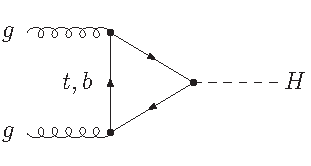
\includegraphics[width=\textwidth]{axodraw/ggF.pdf}
		\caption{Gluon fusion}
		\label{fig:feyn:ggF}
	\end{subfigure}
	\hfill
	\begin{subfigure}[b]{0.3\textwidth}
		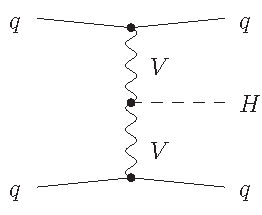
\includegraphics[width=\textwidth]{axodraw/VBF.pdf}
		\caption{Vector boson fusion}
		\label{fig:feyn:VBF}
	\end{subfigure}
	\hfill\null
	\\\bigskip
	\null\hfill
	\begin{subfigure}[b]{0.33\textwidth}
		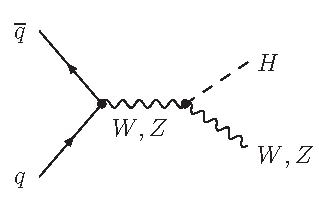
\includegraphics[width=\textwidth]{axodraw/VH.pdf}
		\caption{Higgs-strahlung}
		\label{fig:feyn:VH}
	\end{subfigure}
	\hfill
	\begin{subfigure}[b]{0.25\textwidth}
		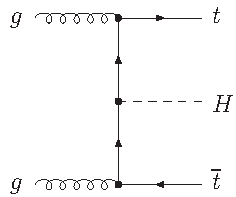
\includegraphics[width=\textwidth]{axodraw/ttH.pdf}
		\caption{Top fusion}
		\label{fig:feyn:ttH}
	\end{subfigure}
	\hfill\null
	\caption{Examples of tree-level Feynman diagrams for the Higgs production processes relevant at the \ac{LHC}.}
	\label{fig:feyn}
\end{figure}

\begin{figure}
	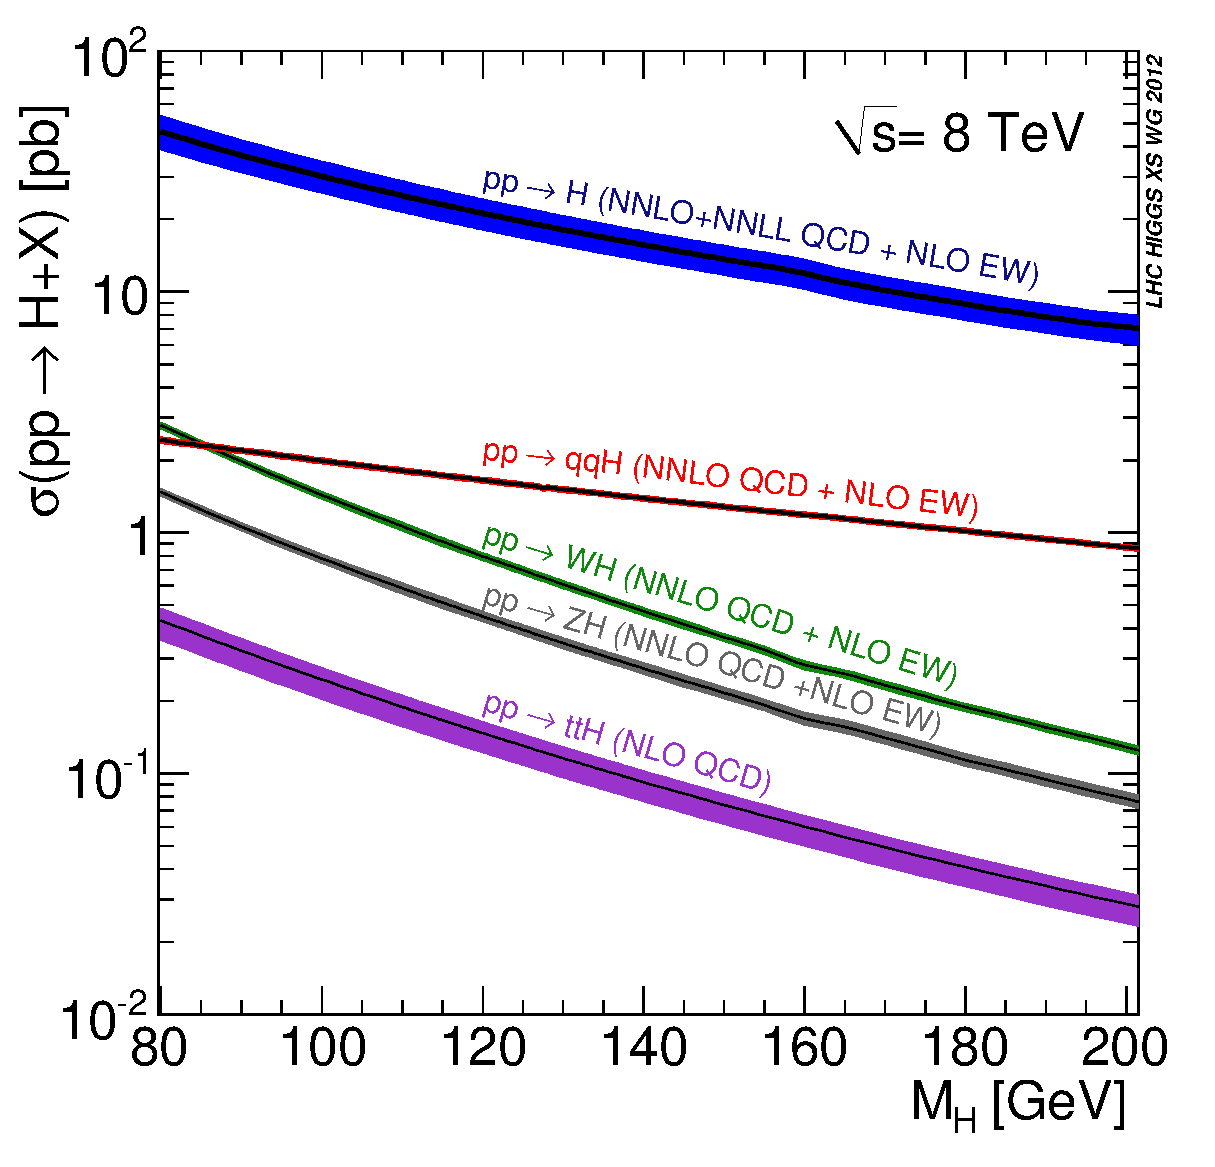
\includegraphics[width=0.48\textwidth]{tex/motivation/xs_lowrange}
	\hfill
	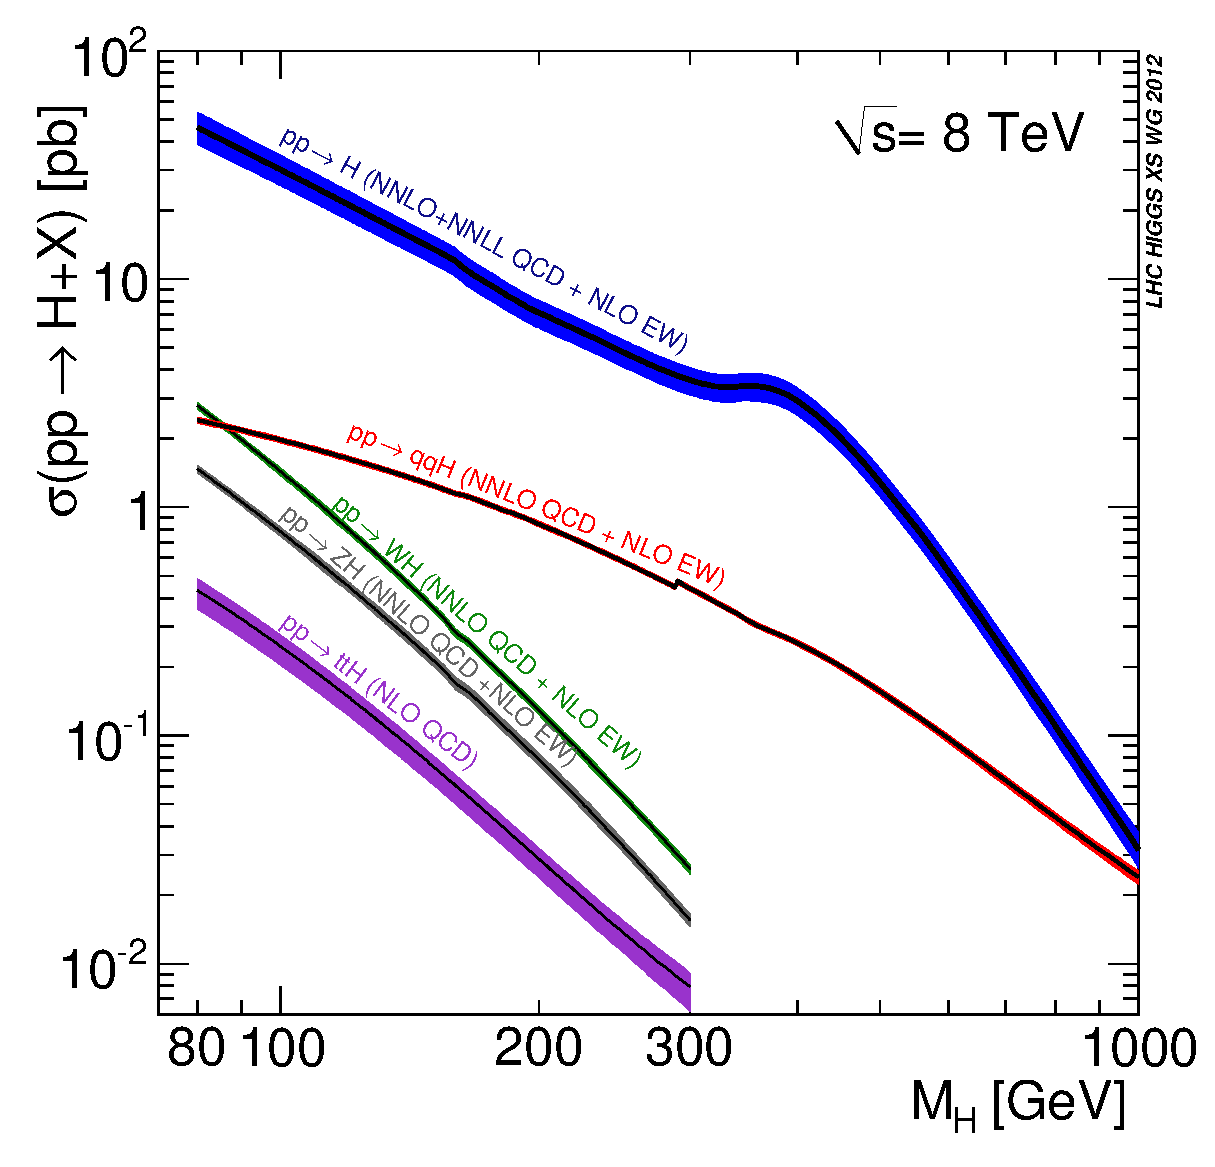
\includegraphics[width=0.48\textwidth]{tex/motivation/xs_fullrange}
	\caption{Cross sections for Higgs boson production versus mass for the low mass range (left) and an expanded mass range (right) \cite{YR2}. Theoretical uncertainties are also displayed. The blue band is \ac{ggF}, the red band is \ac{VBF}, the green band is \WH, the grey band is \ZH and the purple band is \ttH.}
	\label{fig:higgs_xs}
\end{figure}

\begin{figure}
	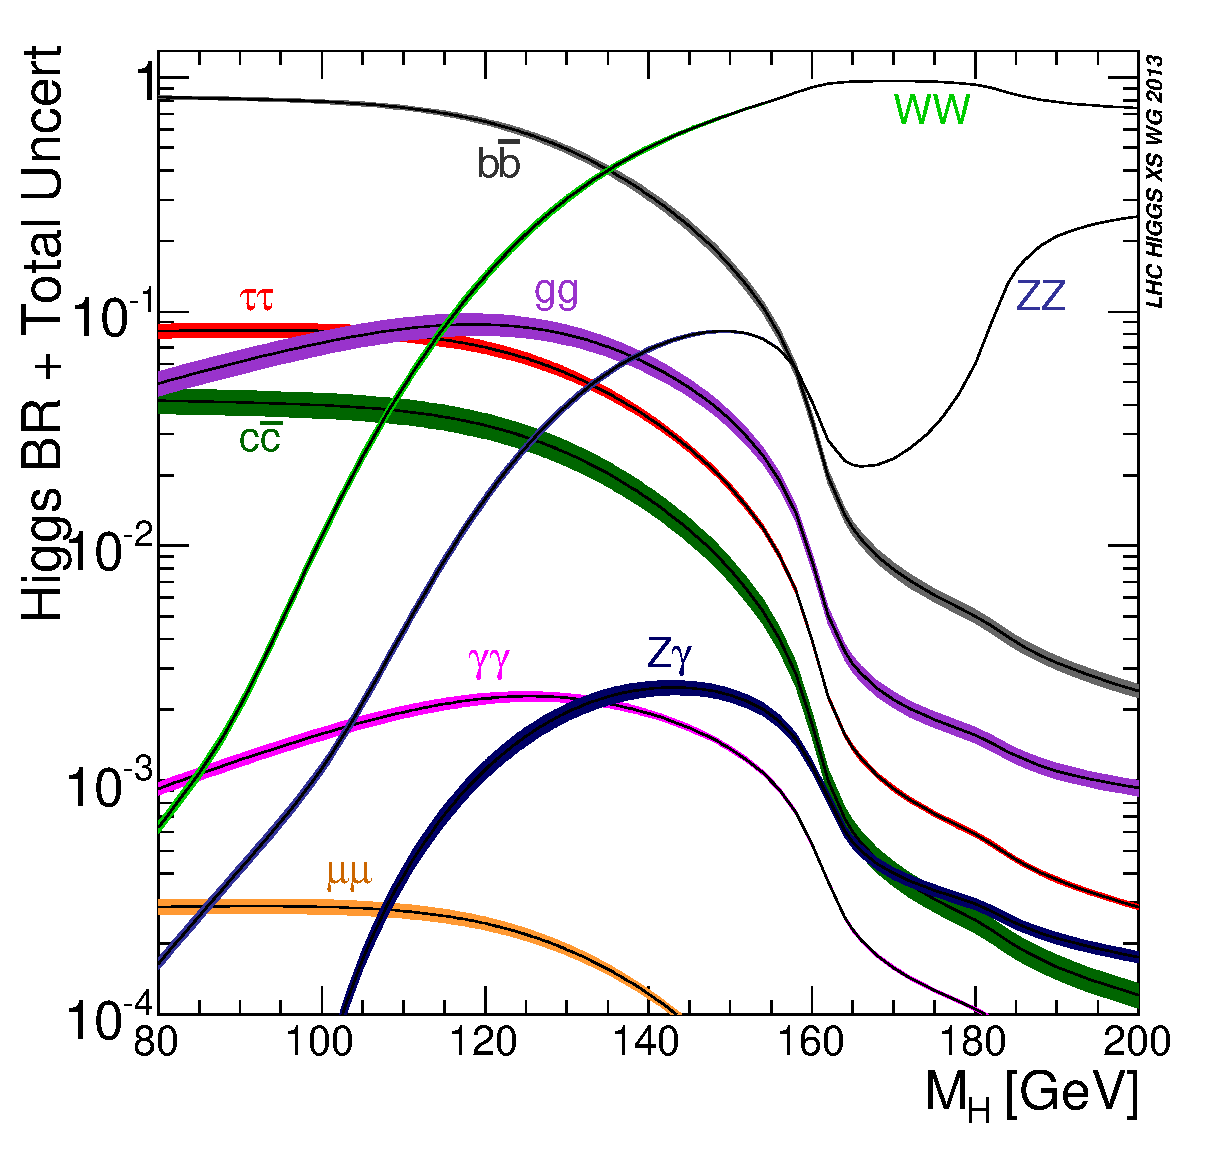
\includegraphics[width=0.48\textwidth]{tex/motivation/BR_lowrange}
	\hfill
	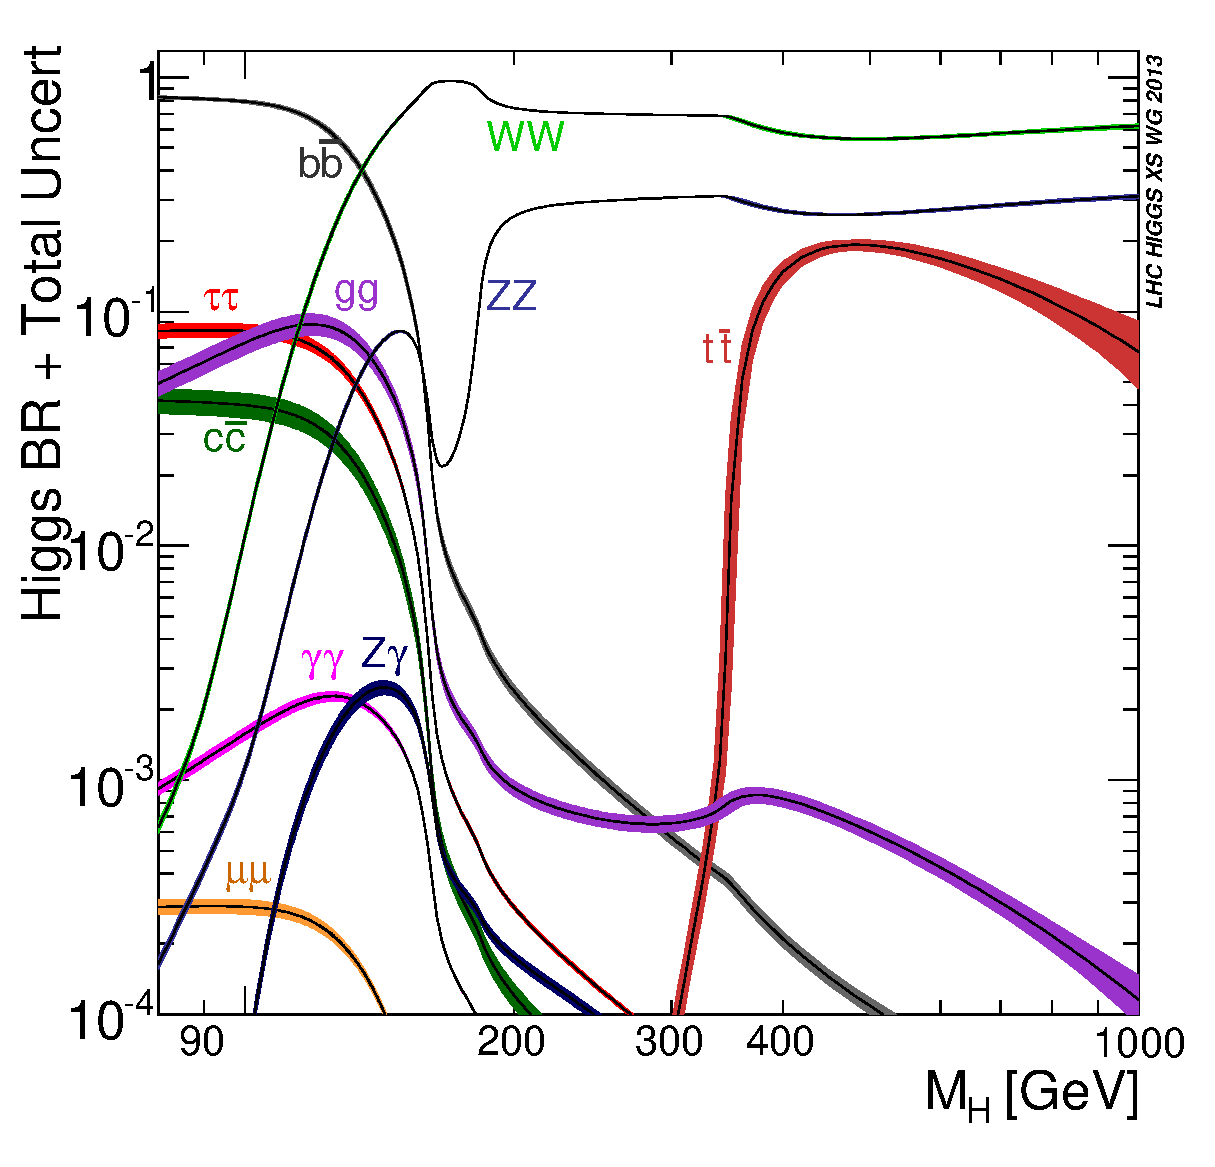
\includegraphics[width=0.48\textwidth]{tex/motivation/BR_fullrange}
	\caption{Branching ratios of the Higgs boson versus mass for the low mass range (left) and an expanded mass range (right) \cite{YR3}. Theoretical uncertainties are also displayed.}
	\label{fig:higgs_br}
\end{figure}
